\documentclass[hidelinks,12pt]{article}
\usepackage[left=0.25cm,top=1cm,right=0.25cm,bottom=1cm]{geometry}
%\usepackage[landscape]{geometry}
\textwidth = 20cm
\hoffset = -1cm
\usepackage[utf8]{inputenc}
\usepackage[spanish,es-tabla]{babel}
\usepackage[autostyle,spanish=mexican]{csquotes}
\usepackage[tbtags]{amsmath}
\usepackage{nccmath}
\usepackage{amsthm}
\usepackage{amssymb}
\usepackage{mathrsfs}
\usepackage{graphicx}
\usepackage{subfig}
\usepackage{standalone}
\usepackage[outdir=./Imagenes/]{epstopdf}
\usepackage{siunitx}
\usepackage{physics}
\usepackage{color}
\usepackage{float}
\usepackage{hyperref}
\usepackage{multicol}
%\usepackage{milista}
\usepackage{anyfontsize}
\usepackage{anysize}
%\usepackage{enumerate}
\usepackage[shortlabels]{enumitem}
\usepackage{capt-of}
\usepackage{bm}
\usepackage{relsize}
\usepackage{placeins}
\usepackage{empheq}
\usepackage{cancel}
\usepackage{wrapfig}
\usepackage[flushleft]{threeparttable}
\usepackage{makecell}
\usepackage{fancyhdr}
\usepackage{tikz}
\usepackage{bigints}
\usepackage{scalerel}
\usepackage{pgfplots}
\usepackage{pdflscape}
\pgfplotsset{compat=1.16}
\spanishdecimal{.}
\renewcommand{\baselinestretch}{1.5} 
\renewcommand\labelenumii{\theenumi.{\arabic{enumii}})}
\newcommand{\ptilde}[1]{\ensuremath{{#1}^{\prime}}}
\newcommand{\stilde}[1]{\ensuremath{{#1}^{\prime \prime}}}
\newcommand{\ttilde}[1]{\ensuremath{{#1}^{\prime \prime \prime}}}
\newcommand{\ntilde}[2]{\ensuremath{{#1}^{(#2)}}}

\newtheorem{defi}{{\it Definición}}[section]
\newtheorem{teo}{{\it Teorema}}[section]
\newtheorem{ejemplo}{{\it Ejemplo}}[section]
\newtheorem{propiedad}{{\it Propiedad}}[section]
\newtheorem{lema}{{\it Lema}}[section]
\newtheorem{cor}{Corolario}
\newtheorem{ejer}{Ejercicio}[section]

\newlist{milista}{enumerate}{2}
\setlist[milista,1]{label=\arabic*)}
\setlist[milista,2]{label=\arabic{milistai}.\arabic*)}
\newlength{\depthofsumsign}
\setlength{\depthofsumsign}{\depthof{$\sum$}}
\newcommand{\nsum}[1][1.4]{% only for \displaystyle
    \mathop{%
        \raisebox
            {-#1\depthofsumsign+1\depthofsumsign}
            {\scalebox
                {#1}
                {$\displaystyle\sum$}%
            }
    }
}
\def\scaleint#1{\vcenter{\hbox{\scaleto[3ex]{\displaystyle\int}{#1}}}}
\def\bs{\mkern-12mu}


\title{Distribución de temperaturas en un cilindro \\ \large {Funciones de Bessel - Tema 5} \vspace{-3ex}}
\author{M. en C. Gustavo Contreras Mayén}
\date{ }

\pagestyle{fancy}
\fancyhf{}
\rhead{Curso MAF}
\lhead{\leftmark}
\rfoot{\thepage}
\setlength{\headheight}{16pt}%

\def\changemargin#1#2{\list{}{\rightmargin#2\leftmargin#1}\item[]}
\let\endchangemargin=\endlist 


\begin{document}
\maketitle
\fontsize{14}{14}\selectfont
\tableofcontents
\newpage

\section{Problema a resolver.}
\subsection{Geometría del problema.}

Se pide calcular la distribución de temperaturas dentro de un cilindro rígido.
\par
Para iniciar bien la solución de cualquier ejercicio, conviene presentar un esquema del problema. En este caso, el cilindro rígido de radio $r = a$, como vemos en la siguiente figura:
\begin{figure}[H]
    \centering
    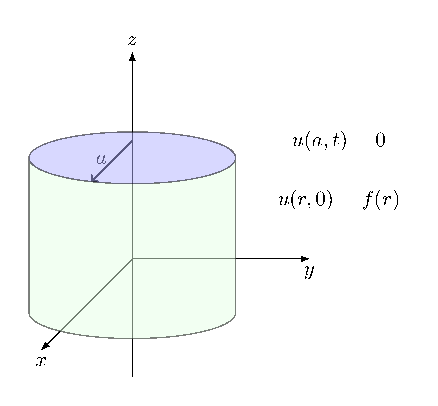
\includegraphics[scale=1]{Imagenes/plot_cilindro_Bessel_01.eps}
\end{figure}

Vemos que no importa la orientación del cilindro, ya sea que lo presentamos de manera horizontal o vertical, el punto importante es considerar que el eje $z$ \enquote{cruza} al cilindro por el centro.

\subsection{Ecuación que modela.}

De acuerdo con lo que nos plantea el enunciado, la ecuación que debemos de ocupar, es la ecuación de calor:
\begin{align}
\pdv{u}{t} = \kappa \left( \pdv[2]{u}{r} + \dfrac{1}{r}  \, \pdv{u}{r} \right) \hspace{1cm} 0 < r < a, \hspace{0.5cm} t > 0
\label{eq:ecuacion_CilBessel_01}
\end{align}
junto con las condiciones:
\begin{align}
u(a, t) = 0 \hspace{2cm} u(r, 0) = f(r)
\label{eq:ecuacion_CilBessel_02}
\end{align}
Debemos de tomar en cuenta que la función $u(r, t)$ (solución) debe de ser acotada en todo el volumen del cilindro.

\subsection{Resolviendo la ecuación.}

Tenemos una EDP lineal y homogénea, por lo que podemos apoyarnos con la técnica de \emph{separación de variables}.
\par
Como la distribución de temperatura no depende  de la parte angular $\theta$, así como del eje $z$, se simplifica el problema. Se propone una solución del tipo:
\begin{align*}
u(r, t) = R(r) \, T(t)
\end{align*}
por lo que se calculan las derivadas parciales $u_{t}$, $u_{r}$ y $u_{rr}$, que vamos a sustituir en la ec. (\ref{eq:ecuacion_CilBessel_01}):
Se tiene entonces que:
\begin{eqnarray*}
\begin{aligned}
u_{t} &= R(r) \, \pderivada{T}(t) \\[0.5em] 
u_{r} &= \pderivada{R}(r) \, {T}(t) \\[0.5em] 
u_{rr} &= \sderivada{R}(r) \, {T}(t)
\end{aligned}
\end{eqnarray*}
que se sustituyen en la ecuación de calor.

Ocupando los valores de las derivadas, la ecuación tiene la forma:
\begin{align*}
R(r) \, \pderivada{T}(t) = \kappa \bigg[ \sderivada{R}(r) \, {T}(t) + \dfrac{1}{r} \, \pderivada{R}(r) \, {T}(t) \bigg]
\end{align*}
Esta expresión la dividimos entre $R(r) \, T(t)$:
\begin{align*}
\dfrac{\pderivada{T}}{T} = \kappa \bigg[ \dfrac{\sderivada{R}}{R} + \dfrac{1}{r} \, \dfrac{\pderivada{R}}{R} \bigg]
\end{align*}
simplificamos la expresión:
\begin{align*}
\dfrac{\sderivada{R} + \dfrac{1}{r} \pderivada{R}}{R} = \dfrac{1}{\kappa} \, \dfrac{\pderivada{T}}{T}
\end{align*}
Cada lado de la igualdad depende de una sola variable, al suponer que éstas son independientes entre sí, la única forma en la que se cumple la expresión, es que debe de ser igual a una constante. La constante de separación será: $-\lambda^{2}$.
\par
La ecuación con la constante de separación es:
\begin{align*}
\dfrac{\sderivada{R} + \dfrac{1}{r} \pderivada{R}}{R} = \dfrac{1}{\kappa} \, \dfrac{\pderivada{T}}{T} = -\lambda^{2}
\end{align*}
Debemos de considerar la condición de frontera $u(a, t) = 0$:
\begin{align*}
R(a) \, T(t) = 0 \hspace{1cm} \Rightarrow \hspace{1cm} R(a) = 0
\end{align*}
Llegamos a un sistema de dos EDO2H:
\begin{align}
\sderivada{R}(r) + \dfrac{1}{r} \, \pderivada{R} + \lambda^{2} \, R(r) &= 0, \hspace{1cm} R(a) = 0 \label{eq:ecuacion_CilBessel_03} \\[0.5em]  
\pderivada{T}(t) + \kappa \, \lambda^{2} \, T(t) &= 0 \label{eq:ecuacion_CilBessel_04}
\end{align}


\section{Propiedades de la función de Bessel.}
\subsection{Identificando la ecuación.}

La ec. (\ref{eq:ecuacion_CilBessel_03}) que es la parte radial del problema:
\begin{align*}
\sderivada{R}(r) + \dfrac{1}{r} \, \pderivada{R} + \lambda^{2} \, R(r) = 0
\end{align*}
es una ecuación de tipo Bessel:
\begin{align*}
\sderivada{y} + \dfrac{1}{x} \, \pderivada{y} + \left( \lambda^{2} - \dfrac{\nu^{2}}{x^{2}} \right) \, y = 0
\end{align*}
Con $\nu = 0$.
Sabemos que la solución general de la ED de Bessel de orden cero es de la forma:
\par
\begin{align*}
R(r) = C_{1} \, J_{0} (\lambda \, r) + C_{2} \, Y_{0} (\lambda \, r)
\end{align*}
con las constantes $C_{1}$ y $C_{2}$ por determinar, $J_{0}$ es la función de Bessel de primer tipo, mientras que $Y_{0}$ es la función de Bessel de segundo tipo (o funciones de Neumann).

\subsection{Constricciones en el problema.}

La función $R(r)$ debe de estar acotada en $r = 0$,  por lo que se deduce que $C_{2} = 0$, ya que:
\begin{align*}
Y_{0}(0) \to \infty
\end{align*}
Por lo tanto:
\begin{align*}
R(r) = C_{1} \, J_{0}(\lambda \, r)
\end{align*}
como $R(a) = 0$, tenemos:
\begin{align*}
C_{1} \, J_{0} (\lambda \, a) = 0
\end{align*}

Se nos presentan dos casos:
\begin{enumerate}[label=\alph*)]
\item El caso trivial con $C_{1} = 0$.
\item El caso no trivial: $C_{1} \neq 0$, así:
\begin{align}
J_{0} (\lambda \, a) = 0
\label{eq:ecuacion_CilBessel_05}
\end{align}
\end{enumerate}

\subsection{Soluciones a las EDO.}

Si $\lambda_{i} = 1, 2, \ldots$ son las raíces positivas (eigenvalores) de la ec. (\ref{eq:ecuacion_CilBessel_05}), se tiene que aparte del factor constante, las funciones:
\begin{align*}
R_{i}(r) = J_{0} (\lambda_{i} \, r) \hspace{1.5cm} i = 1, 2, \ldots
\end{align*}
son soluciones a la EDO2H radial, ec. (\ref{eq:ecuacion_CilBessel_03}), es decir, son las eigenfunciones.
\par
Para los valores $\lambda$ considerados, la ec. (\ref{eq:ecuacion_CilBessel_04}), es decir, la parte temporal tiene las soluciones particulares:
\begin{align*}
T_{i} (t) = \exp(-\kappa \, \lambda_{i}^{2} \, t) \hspace{1.5cm} i = 1, 2, 3, \ldots
\end{align*}
La sucesión de funciones que son la solución completa:
\begin{align*}
u_{i}(r, t) = C_{i} \, J_{0} (\lambda_{i} \, r) \, \exp(-\kappa \, \lambda_{i}^{2} \, t) 
\end{align*}
satisfacen la ec. (\ref{eq:ecuacion_CilBessel_01}) así como la condición de frontera. De acuerdo con el principio de superposición, la función:
\begin{align}
u(r, t) = \nsum_{i=1}^{\infty} C_{i} \, J_{0} (\lambda_{i} \, r) \, \exp(-\kappa \, \lambda_{i}^{2} \, t)
\label{eq:ecuacion_CilBessel_06}
\end{align}
también satisface a la ecuación de calor inicial y la CDF. Ocupando la condición:
\begin{align*}
u(r, 0) = f(r)
\end{align*}
se obtiene la serie de Fourier-Bessel:
\begin{align}
f(r) = \nsum_{i=1}^{\infty} C_{i} \, J_{0}(\lambda_{i} \, r)
\label{eq:ecuacion_CilBessel_07}
\end{align}
quedando por determinar los coeficientes $C_{i}$.  Para obtener esos coeficientes, haremos un breve repaso sobre las series de Fourier-Bessel.

\subsection{Series de Fourier-Bessel.}

Supongamos que una función $f(x)$ tiene un desarrollo convergente de la forma:
\begin{align}
f(x) = \nsum_{i=1}^{\infty} C_{i} \, J_{\nu} (\lambda_{i} \, x) \hspace{1cm} 0 < x < a
\label{eq:ecuacion_CilBessel_08}
\end{align}
donde los $\lambda_{i}$ con $i = 1, 2, \ldots$ son las raíces positivas de $J_{\nu} (\lambda \, a) = 0$. Multiplicamos ambos lados de la ec. (\ref{eq:ecuacion_CilBessel_08}) por $x \, J_{\nu}(\lambda_{j} \, x)$ con $j$ fijo, para luego integrar entre $0$ y $a$, suponiendo que la serie es integrable término a término, llegando a:
\begin{align*}
\scaleint{6ex}_{\bs 0}^{a} &x \, f(x) J_{\nu}(\lambda_{j} x) \dd{x} = \\[0.5em]
&= \nsum_{i=1}^{\infty} C_{i} \scaleint{6ex}_{\bs 0}^{a} x \, J_{\nu} (\lambda_{i} x) \, J_{\nu} (\lambda_{j} x) \dd{x}
\end{align*}
Para resolver la integral del lado derecho:
\begin{align*}
\scaleint{6ex}_{\bs 0}^{a} x \, J_{\nu} (\lambda_{i} x) \, J_{\nu} (\lambda_{j} x) \dd{x}
\end{align*}
habrá que emplear la propiedad de ortogonalidad de las funciones de Bessel.
\par
Sabemos que las funciones de Bessel cuentan con la propiedad de ortogonalidad, dada por la expresión:
\begin{align*}
\scaleint{5ex}_{\bs 0}^{a} &x \, J_{\nu} (\lambda_{i} \, x) \, J_{\nu} (\lambda_{j} \, x) \dd{x} = \\[1em]
&= \begin{cases}
0 & i \neq j \\
\dfrac{a^{2}}{2} \, \big[ J_{\nu+1} (\lambda_{i} \, a)\big]^{2} & i = j, \hspace{0.5cm} i = 1, 2, \ldots
\end{cases}
\end{align*}
Los coeficientes $C_{i}$ son entonces:
\begin{eqnarray*}
\begin{aligned}
C_{i} &= \dfrac{\scaleint{5ex}_{\bs 0}^{a} x \, f(x) \, J_{\nu}(\lambda_{i} \, x) \dd{x}}{\scaleint{5ex}_{\bs 0}^{a} x \, \big[ J_{\nu} (\lambda_{i} \, x) \big]^{2} \dd{x}} \hspace{1cm} i = 1, 2, \ldots \\[1em] 
&= \dfrac{\scaleint{5ex}_{\bs 0}^{a} x \, f(x) \, J_{\nu}(\lambda_{i} \, x) \dd{x}}{\dfrac{a^{2}}{2} \, \big[ J_{\nu+1}^{2} (\lambda_{i} \, a) \big]} \hspace{1cm} i = 1, 2, \ldots
\end{aligned}
\end{eqnarray*}
Por lo tanto, los coeficientes $C_{i}$ quedan definidos por la expresión:
\begin{align*}
C_{i} = \dfrac{2}{a^{2}} \dfrac{\scaleint{5ex}_{\bs 0}^{a} x \, f(x) \, J_{\nu}(\lambda_{i} \, x) \dd{x}}{ \big[ J_{\nu+1} (\lambda_{i} \, a) \big]^{2}} \hspace{1cm} i = 1, 2, \ldots
\end{align*}
Con este resultado, ya podemos regresar al ejercicio y definir la solución completa al problema.

\subsection{Regresando a la solución.}

Con acuerdo a la manera en que se obtuvieron los coeficientes $C_{i}$ de una serie de Fourier-Bessel, para el problema del cilindro, se tiene que:
\begin{align}
\begin{aligned}
C_{i} = \dfrac{2}{a^{2} \, \big[ J_{1} (\lambda_{i} \, a) \big]^{2}} &\scaleint{6ex}_{\bs 0}^{a} r \, f(r) \, J_{0}(\lambda_{i} \, r) \dd{r} \\[0.5em]
i &= 1, 2, \ldots
\end{aligned}
\label{eq:ecuacion_Cil_Bessel_09}
\end{align}

La distribución de temperaturas en el cilindro viene dada por la expresión:
\begin{eqnarray}
\begin{aligned}[b]
u(r, t) &= \dfrac{2}{a^{2}} \nsum_{i=1}^{\infty} \bigg[ \, \scaleint{6ex}_{\bs 0}^{a} \, r \, f(r) J_{0} (\lambda_{i} \, r) \dd{r} \bigg] \, \dfrac{J_{0} (\lambda_{i} \, r)}{\big[ J_{1} (\lambda_{i} \, a) \big]^{2}} \, \exp( -\kappa \, \lambda_{i}^{2} \, t)
\end{aligned}
\label{eq:ecuacion_CilBessel10}
\end{eqnarray}
donde la suma es tomada sobre todas las raíces positivas de la ec. (\ref{eq:ecuacion_CilBessel_05}).
\end{document}